\documentclass[oneside,openany]{bjtuThesis}
\usepackage{graphicx}
\usepackage{amsmath}
\usepackage{mathptmx}
\usepackage{float}
\usepackage[numbers,square]{natbib}
%\bibliographystyle{plainnat}
\newcommand\mycite[1]{{\setcitestyle{square,super}\cite{#1}}}
\newcommand\mycitex[1]{{\setcitestyle{authoryear,round}\cite{#1}}}
%\usepackage{algorithm}
%\usepackage{algorithmic}
\usepackage[ruled,linesnumbered,noend]{algorithm2e}
\usepackage{fontspec}
\setmainfont{Times New Roman}
\usepackage{cases}  
%\usepackage{mathtools}
\usepackage{amssymb}
\usepackage{multirow}
\hypersetup{colorlinks,linkcolor=red,citecolor=black,urlcolor=magenta}% 链接颜色设置
\linespread{1.5}% 设置行距
%-------------------------------------------------------------------------------
%                加载宏包
%-------------------------------------------------------------------------------
% 示例:\usepackage{amsmath}% 加载宏包
%-------------------------------------------------------------------------------
%                论文的基本信息
%-------------------------------------------------------------------------------
% 论文中文标题(36个汉字以内)
\ctitle{\textbf{基于脉冲神经网络的物体检测}}

% 论文英文标题(72个字符以内,包含空格)
\etitle{Object detection based on spiking neural network}

% 姓名(10个汉字以内)
\author{何翔}

% 学号
\studentid{17292012}

% 学院,依次为学院全称(10个汉字以内),学院简称(2个汉字以内)
\school{电子信息工程学院}{电信}

% 专业,依次为专业全称(10个汉字以内),专业简称(2个汉字以内)
\major{轨道交通信号与控制}{信号}

% 导师(10个汉字以内)
\mentor{}

% 封面的日期,依次为年,月,日
\coverdate{2021}{04}

%bjtu
\bjtu{北京交通大学}% 加载论文信息

\begin{document}

% 封面
\makecover
\makeAuthorization
\frontmatter
\thesispagestyle{-4}{北京交通大学毕业设计(论文)}{}% 页眉设置

% 中文摘要
%-------------------------------------------------------------------------------
%                中文摘要
%-------------------------------------------------------------------------------
\cabstract
{
中文摘要。\par
中文摘要!
}
{\quad 关键词1 \quad 关键词2}


% 英文摘要
%-------------------------------------------------------------------------------
%                英文摘要
%-------------------------------------------------------------------------------
\eabstract
{
Abstract.\par
Abstract!
}
{\quad keyword1 \quad keyword2}

% 目录
\tableofcontents

\mainmatter
\thesispagestyle{-4}{北京交通大学毕业设计(论文)}{第 \thepage 页}% 页眉设置

% 正文
\chapter{引言}
\section{研究背景}
\par
目标检测是一种应用特定计算机算法在图像中找到所需目标的技术。
近年来,随着计算机硬件的不断发展,目标检测的各种算法也迎来了巨大的突破
,越来越多地应用于交通检测、智能支付、医疗影像等各个方面。
在计算机视觉中,目标检测是要比图像分类更复杂的一个问题,它不仅要清楚目标的类型,还需做到目标的定位。
所以,物体检测的难度更大,挑战性更强,相应的深度学习模型也会更加复杂。
\par
目标检测有许多算法,卷积神经网络(Convolutional Neural Networks, CNN)
是其代表算法之一。它是一个前馈神经网络,具有卷积计算和深度结构。
目前,基于卷积神经网络的目标检测算法大致可分为两种模式,
即 two-stage 模式和 one-stage 模式,
two-stage模式的检测过程分为两个步骤:首先由算法生成若干个候选框,
再通过CNN对候选框进行分类;
one-stage模式则是端到端的学习,直接对对目标的置信概率和位置进行回归,
相对来说精度有所损失,但速度较two-stage模式的算法更快。\mycite{2020基于卷积神经网络的目标检测综述}
\par
基于two-stage的算法有:
\begin{itemize}
    \item R-CNN:通过选择性搜索(selective search)来确定候选框,之后统一将候选框压缩到大小;
    然后运用CNN对候选框进行特征提取;最后使用多个支持向量机(SVM)分类器分类输出向量,
    采用边界回归生成目标区域\mycite{R-CNN}。
    \item Fast R-CNN:仍然使用选择性搜索来确定候选框,但将整张图片输入到CNN,
    在卷积特征层上使用感兴趣区域(Region of interest pooling,ROI pooling)操作,
    并从特征图中提取一个特定长度的特征向量;然后将特征向量输入到全连接层,
    用softmax对其进行分类;最后对属于同一特征的候选框进行分类并回归其位置\mycite{FastR-CNN}。
    \item Faster R-CNN:使用 RPN (Region Proposal Network)而不是选择性搜索,大大减少了提取候选框的时间。
    将 RPN 和 Fast R-CNN 相结合,首先提取整张图片的特征;再将特征结果输入到 RPN;
    然后使用 ROI 池化层固定候选框的大小;最后对属于某一特征的候选框回归和调整\mycite{FasterR-CNN}。
\end{itemize}
\par
基于one-stage的算法有:
\begin{itemize}
    \item YOLO v1和许多后续的改进算法:
    YOLO 系列算法是目前一种先进的目标检测算法。
    因为整个检测框架是一个整体,所以可以端到端地对算法的性能进行优化。
    \item SSD系列算法:采用多尺度特征图用于检测.,设置先验框,采用卷积进行检测。
\end{itemize}
\par
脉冲神经网络(Spiking Neural Network, SNN),起源于脑科学,由于其丰富的时空领域的神经动力学特性、多样的编码机制和超低的功耗被誉为第三代神经网络。在此之前,神经网络经历了几个发展阶段:
第一个阶段是感知机阶段,其可以模拟人类感知能力并由美国神经学家 Frank Rosenblatt在BM704机上完成了仿真。
第二个阶段是基于联结主义的多层人工神经网络 (Artificial Neural Network, ANN),其兴起于二十世纪 80 年代中期。20世纪80年代末,分布式表达与反向传播算法被提出。
在2006年以后,深度卷积网络占有重要地位,引领了近十几年人工智能的发展\mycite{2021脉冲神经网络研究进展综述}。
\par
ANN各个深度学习领域(如计算机视觉和自然语言处理)取得了巨大的成功,但ANN在生物学上是不精确的,不能较准确地模仿生物大脑神经元的运作机制,缺乏一定的生物可解释性。为了使神经网络更加接近于人脑,SNN随之诞生。但与ANN在各方面的广泛应用不同,SNN领域仍有许多问题有待解决,其研究仍然处于快速发展的早期阶段。
\section{研究意义}
\par
SNN作为第三代人工神经网络,基于神经动力学的事件驱动机制,使得其擅长高效处理复杂、稀疏的时空信息。并且SNN在硬件电路上具有超低能耗实现的优势。
2019年清华大学研制的ANN/SNN异构融合天机芯登上Nature封面,指出计算机科学导向的深度学习和神经科学导向的脉冲神经网络的交叉融合将是人工通用智能的发展方向\mycite{2019Towards}。
\par
本设计论文研究的意义在于探索脉冲神经网络在目标检测上的应用,目前主流的脉冲神经网络训练算法有直接BP训练、STDP无监督训练和训练好的ANN的转化,
虽然训练算法众多,但是SNN仍然没有一套成熟的训练算法。比如在较大较深的网络训练中,面临着脉冲信号的编码问题、训练开销大等问题\mycite{2021脉冲神经网络研究进展综述}。
并且在实现目标检测上,需要更为复杂的网络结构,目前公开的检测方法也只有\mycitex{Spiking-yolo}等人在经典的YOLO模型上进行转化的spiking-yolo。为此,基于不同的网络结构实现SNN,以方便实现在硬件上的低功耗,并与已有结果进行对比,是有一定意义的。
\section{论文组织与结构}
\par
本文的研究内容是:在总结和分析国内外ANN进行转化的SNN的理论基础上,利用现有的ANN目标检测模型,分析转化过程中存在的损失,以及各种转化手段的实现方式;同时对转化模型和前人做的工作做对比,分析不同模型对SNN转化的影响,并在pytorch框架下对模型进行设计与实现。
\par
本文以问题提出引申到理论支持,再到算法研究及具体的解决方案设计为思路进行组织,共分为以下六章:
\par
第一章为本章:首先阐述脉冲神经网络与目标检测研究的背景和意义,然后提出了本文研究的主要内容为设计转换模型并与前人工作做对比分析不同模型对SNN转换的影响,最后给出了论文的结构与框架。
\par
第二章系统介绍了脉冲神经网络:发展趋势、优缺点、学习方法等。重点对从ANN到SNN转换的方法进行了阐述
\par
第三章给出了目标检测中常用的人工神经网络模型(Artificial Neural Network,ANN),以one-stage代表算法SSD为例,对模型的结构、损失函数等方面进行阐述。
\par
第四章介绍模型的设计思路与方法
\par
第五章结合实验,分别进行ssd,spiking-ssd的对比;yolo,spiking-yolo的对比。给出实验结果,进行分析。
\par
第六章总结分析,从多个角度对转换模型现有结果进行分析,并给出了产生这种结果的可能原因。
\chapter{脉冲神经网络}
\par
在过去多年中,人工神经网络(ANN)已能够解决很多问题。但当我们尝试解决更高级的问题时,对算力和电源的不断增长的需求是不可避免的,在可用资源有限的嵌入式系统上几乎不可能采用ANN。
鉴于这些情况,由于事件驱动性和低功率特性,脉冲神经网络(SNN)作为第三代神经网络正在引起广泛关注。然而,SNN的复杂的动态神经元和不可微分的脉冲操作给其带来了显著的性能下降。因此,其应用仅限于相对简单的任务,例如图像分类。
在最近的研究中,Seijoon Kim等人研究了SNN在更具挑战性的对象检测任务中的性能下降\mycite{Spiking-yolo},并提出了第一个用于目标检测的脉冲神经网络模型Spiking-yolo,该模型是对现有的yolo模型进行转化,因此下文中先简述脉冲神经网络的各种学习算法,再重点对转化的方法进行阐述。
\section{学习算法}
\par
人工神经网络的学习是根据数据对网络的关键参数进行调整和优化的过程。
优化学习算法在这一过程中起着至关重要的作用。
目前人工神经网络优化理论中,结合误差反向传播的梯度下降算法是其核心。
\par
相比之下,当前脉冲神经网络领域还没有成熟的训练算法。网络采用的神经元模型和编码方式各异,均造成了训练算法的多样化。
总体来讲,主流的实现SNN的方式有三种:第一种是基于STDP等生物解释性好的算法进行训练,第二种是直接使用BP算法进行反向传播,这实现起来也相对困难。第三种是运用成熟的人工神经网络,对其进行转换,
也可以按是否采用标签信息将其分为无监督学习和有监督学习两类。脉冲神经网络一些常用的学习算法如下图\mycite{2021脉冲神经网络研究进展综述}所示:
\begin{figure}[htbp]
	\centering
	\setlength{\abovecaptionskip}{0cm}  
	\setlength{\belowcaptionskip}{0cm}
	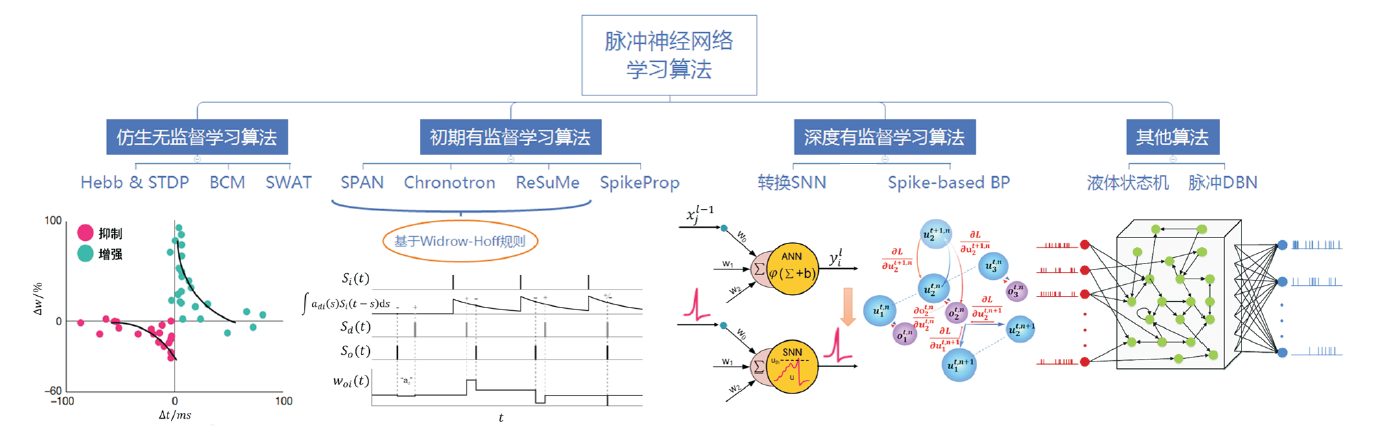
\includegraphics[width=1\textwidth]{figures/study.png}
	\caption{常见的SNN学习算法}
\end{figure}
\section{ANN转化的SNN}
\par
转化SNN (ANN-converted SNN) 是为了在已发展出的深度学习成果上,与硬件结合从而进一步利用事件驱动特性的低能耗优势,从ANN的视角出发的一种SNN实现方法。其作为间接监督性学习算法,
基本理念是在使用ReLU函数的ANN网络中, 用SNN中频率编码下的平均脉冲发放率来近似ANN中的连续激活值。完成原始ANN训练后, 再通过特定的结构将其转换为SNN. 
实质上, 转换SNN的训练依赖的仍是在ANN中进行的反向传播算法, 但是因为没有直接训练SNN的困难. 所以就性能表现而言, 转换SNN保持着与ANN很小的差距, 这一点在大的网络结构和数据集上的良好表现得到了印证\mycite{rueckauer2016theory}。
\subsection{国内外研究进展}
\par
关于ANN-to-SNN转换的早期研究始于\mycitex{2013Conversion}等人的工作。其中CNN单元被取代成具有泄漏和不应期的生物启发的脉冲单元,旨在处理来自基于事件流的输入。\mycitex{Cao2014SpikingDC}等人提出了脉冲神经元传递函数之间的紧密联系,即输入电流和输出发放频率与整流线性单元(ReLU)之间的关系,这是当今人工神经网络中神经元的标准模型。Diehl等人改进了他们的方法。通过使用权重归一化方案,对MNIST\mycite{Lecun}分类任务实现了几乎无损失的人工神经网络转换。该技术重新调整权重以避免由于神经元的过多或过少而导致的SNN中的近似误差。
\mycitex{2016Hun}引入了一种转换方法,其中训练期间的噪声注入通过更逼真的生物神经元模型提高了对SNN的近似误差的鲁棒性。\mycitex{Esser_2016}等演示了一种为TrueNorth平台优化CNN的方法,该平台具有二进制权重和受限连接。\mycitex{zambrano2016fast}开发了一种使用尖峰神经元的转换方法,该神经元适应其环形阈值以减少编码信息所需的尖峰数量。
这些方法在MNIST上取得了非常好的结果,但是当扩展到可以解决CIFAR-10\mycite{Krizhevsky09learningmultiple}的网络时,SNN结果低于最先进的ANN结果。一个原因是,对于提高ANN误差率至关重要的许多运算符的SNN实现(例如最大池化层,softmax激活函数和批量归一化)是不存在的,因此SNN只能近似地匹配ANN的推断。因此,下文中给出一些转化的具体方案和理论知识。
\subsection{脉冲发放率和模拟激活值数学分析}
\par
我们假设ANN单元和SNN神经元之间存在一对一的对应关系,对于具有$L$层的网络,让$\mathbf{W}^l,l \in {1,...,L}$表示连接单元$1-1$至层$l$中的单元的重量矩阵,偏置为$\mathbf{b}^l$。每层中的单元数是$M^l$。层$l$中连续值神经元$i$的ReLU激活计算如下:
\[
a_i^l:= max \Biggl(0,\sum\limits_{j=1}^{M^{l-1}}W_{ij}^la_j^{l-1} + b_i^l \Biggr)
\]\par
每个SNN神经元都具有膜电位$V_i^l(t)$,它在每个时间步长积分其输入电流:
\[
z_i^l(t):= V_{thr} \Biggl(\sum\limits_{j=1}^{M^{l-1}}W_{ij}^l\Theta_{t,j}^{l-1} + b_i^l \Biggr)
\]\par
此处$V_{thr}$是阈值并且$\Theta_{t,j}^{l}$是时间$t$内发放脉冲的阶跃函数
\begin{equation}
	\Theta_{t,j}^{l}= \Theta(V_i^l(t-1) + Z_i^l(t) - V_{thr}),\text{with }
	\Theta(x) = 
	\begin{cases}
		1, & \text{if } x \ge 0; \\
		0, & \text{else.}
	\end{cases}
\end{equation} \par
每个SNN神经元$i$的发放率可以由下计算
\[
\setlength\abovedisplayskip{1pt}
\setlength\belowdisplayskip{1pt}
r_i^l(t):=N_i^l(t)/t
\]\par
其中$N_i^l(t)=\sum_{t'=1}^t\Theta_{t',i}^l$,即脉冲的产生数\par
神经元对输入$z_i^l(t)$进行积分直到膜电势$V_i^l(t)$超过阈值$V_{thr}$,产生脉冲。复位的方式有两种,一种是Diehl等人使用的将膜电势设置为基线,通常为零;另一种是通过减法的复位,在超过阈值时,从膜电势中减去阈值$V_{thr}$。通过减法机制简单地切换到复位可以改善近似,并使转换方案也适用于更深的网络。多余的电荷ǫ在复位时不会被丢弃,可以用于下一个脉冲生成。所以我们优先采用减法重置的方式。\par
对归一化的网络,假定输入恒定为$z \in [0,1]$,对采用减法重置的IF神经元,其膜电势随时间变化为
\[
V_i^l(t) = V_i^l(t-1) + z_i^l(t) -V_{thr}\Theta_{t,i}^l
\]
由前式$Z_i^l = V_{thr}a_i^l$,对T时间步内膜电位进行求和:
\[
\sum\limits_{t=1}^T V_i^l(t) = \sum\limits_{t=1}^T V_i^l(t-1) + z_i^l(t)T - V_{thr}\sum\limits_{t=1}^T\Theta_{t,i}^l
\]\par
移项并且两边同时除$T$
\[
\frac{\sum\limits_{t=1}^T V_i^l(t)-\sum\limits_{t=1}^T V_i^l(t-1)}T = V_{thr}a_i^l - V_{thr}\frac{\sum\limits_{t=1}^T\Theta_{t,i}^l}T
\]
即
\[
r_i^t(t)=a_i^l-\frac{\sum\limits_{t=1}^T V_i^l(t)-\sum\limits_{t=1}^T V_i^l(t-1)}{TV_{thr}}
\]
故在仿真时间步长$T$无限长情况下:
\[
r_i^l(t) = a_i^l(a > 0)
\]
\section{ANN操作的脉冲实现}
\subsection{偏置}
\par
以前提出的SNN转换方法中,因为神经网络的偏置很难表示,所以简单地将其设置为0。在脉冲神经网络中,也可以简单地用比例于偏置的恒定输入流进行表示。 但一些负偏置不得不使用颠倒神经元符号的方式来表示。
\subsection{参数标准化}
\par
Diehl等人引入了权重标准化作为避免由于过低或过高的发放率引起的近似误差的手段。除此之外还有一些其他的归一化方法,在改善转换后SNN的性能
\subsubsection{偏差归一化}
\par
基于数据的权重归一化机制基于ANN的ReLU单元的线性,通过线性地重新调整所有权重和偏差,可以简单地将其扩展到偏差,使得对于所有训练示例,ANN激活a小于1.为了保留层内编码的信息,需要同时缩放一层的参数.将层中的最大ReLU激活表示$\lambda^l=\text{max}[\mathbf{a}^l]$,然后将权重$\mathbf{W}^l$和偏差$\mathbf{b}^l$归一化为$\mathbf{W}^l \to \mathbf{W}^l \frac{\lambda^l}{\lambda^{l-1}}$和$\mathbf{b}^l \to \mathbf{b}^l / \lambda^l$。 

\subsubsection{除异常值归一化}
\par
虽然权重归一化避免了SNN中的发放率饱和,但它可能导致非常低的发放率,从而增加了延迟,直到信息到达更高层。我们将前一段中描述的算法称为“max-norm”,因为归一化因子$\lambda^l$被设置为层内的最大ANN激活,其中使用训练数据的大子集来计算激活。这是一种非常保守的方法,可确保SNN发放率最有可能不超过最大发放率。缺点是该程序易于受到导致非常高的激活的单个异常值样本的影响,而对于大多数剩余样本,该发放率将远低于最大发放率。
\par
因此在实际进行归一化时,我们设置一个百分位数p,称为“归一化标度”,并注意“max-norm”方法在特殊情况p = 100时被恢复。p表现良好的典型值在[99.0,99.999]范围内。引入p的目的就是为了防止除以个别过大的值,导致较低的发放率
\subsection{BN层的转化}
\par
ANN为了快速训练和收敛提出了批归一化(Batch Normalization),批归一化旨在将ANN输出归一化到0均值,这与SNN的特性相违背。因此,需要将BN的参数吸收到前面的参数层中。训练后,这些变换可以整合到权重向量中,从而保留BN的效果,但不需要在推理期间对每个样本重复计算归一化对于给定的网络,这只需要进行一次;在推理期间,参数不会改变。
\par
假定BatchNorm的参数为$\gamma$ (BatchNorm.weight),$\beta$ (BatchNorm.bias),$\mu$ (BatchNorm.mean),$\sigma$ (BatchNorm.var):这四个参数都是在训练期间获得的。参数模块具有参数 $W$ 和 $b$ 。BatchNorm参数吸收就是将BatchNorm的参数通过运算转移到参数模块的 $W$
中,使得数据输入新模块的输出和有BatchNorm时相同。 对此,新模型的$\bar{W}$ 和 $\bar{b}$ 公式表示为:
\[
\bar{W} = \frac{\gamma}{\sigma}W
\]
\[
\bar{b} = \frac{\gamma}{\sigma}(b-\mu) + \beta
\]
\subsection{脉冲层中的最大池化}
\par
大多数\mycite{8594067}成功的人工神经网络使用最大池化来空间下采样特征图。然而,这还没有在SNN中使用。一些现有的方法是基于先到时间脉冲编码,即第一个发放脉冲的神经元被认为是最大的神经元。还有一些简单的脉冲池化机制:输出单元包含门控函数,只允许来自最大神经元的脉冲通过,同时丢弃来自其他神经元的脉冲。
\chapter{ANN模型结构}
\par
目前,目标检测中two-stage系列模型基本采用以下的流程:假设物体边框,对每个边框内进行特征再采样,最后使用分类器进行分类。
这个流程比较流行,但它们存在一个问题:虽然检测效果都很好,但是这些方法对于设备来说计算量过大,甚至需要高端硬件的支持,
对于实时系统来说太慢。最快的检测器也没有到我们理想的速度。考虑后续作为SNN转化的基础模型,我们选择速度较快的单阶段检测器。
\par
下面先介绍SSD算法---多类别单阶段检测器。SSD的设计为端到端训练,精度高,甚至在低分辨率的图像上效果也不错。
其设计理念可总结为:
(1)采用多尺度特征图用于检测(较大的特征图检测小目标,小的特征图检测大目标)
(2)采用卷积进行检测
(3)设置先验框(减小训练难度)。
下面对网络结构进行详细介绍
\section{SSD}
\subsection{基础网络}
\par
我们首先放出SSD的网络结构,如下图\mycite{2016SSD}所示:
\begin{figure}[htbp]
	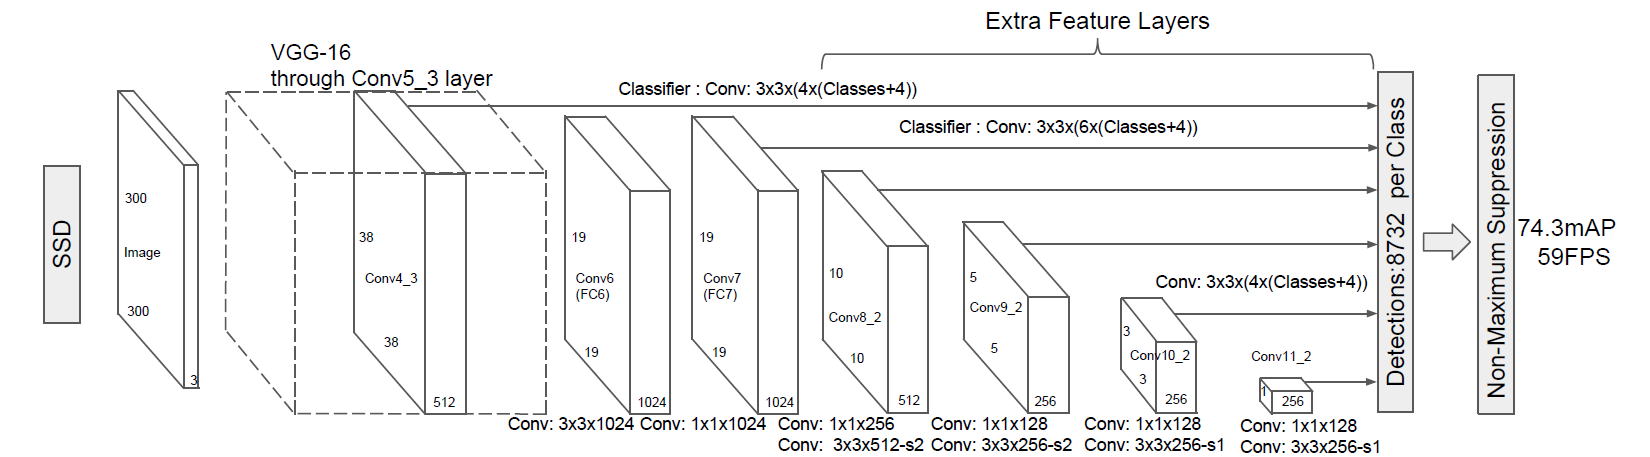
\includegraphics[width=1\textwidth]{figures/ssdnet.png}
	\setlength{\abovecaptionskip}{0cm}  
	\setlength{\belowcaptionskip}{0cm}  
	\caption{ssd网络结构}
\end{figure}
\par
可以看到原始的SSD网络是以VGG-16作骨干网络(Backbone)的,SSD从六个卷积层上提取信息,所用到的特征图以及大小如下表所示:
\par
{
\begin{center}
\begin{tabular}{|rr|}
	\hline
	feature map & 大小\\
	\hline
	Conv4\_3 & 38*38\\
	Conv7 & 19*19\\
	Conv8\_2 & 10*10\\
	Conv9\_2 & 5*5\\
	Conv10\_2 & 3*3\\
	Conv11\_2 & 1*1\\
	\hline
\end{tabular}
\end{center}
}
\par
SSD一共有6层多尺度提取的网络,每层分别对 loc 和 conf进行卷积,得到相应的输出。以conv4\_3为例:
\begin{figure}[!ht]
	\centering
	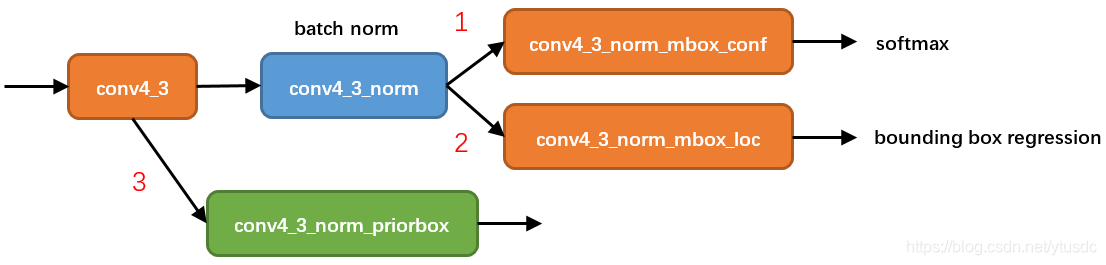
\includegraphics[width=1\textwidth]{figures/conv43.png}
	\caption{单个特征层的特征提取}
\end{figure}
\par
经过conv4\_3层之后,网络分为了3条路线:一是用于softmax分类目标和背景,计算置信度的特征层;二是用于边界框预测的回归层;
三是用于生成并保留先验框位置信息。目标检测中的分类加定位,就是分别由分类层和回归层实现。其中一个细节是这里只有conv4\_3层
进行了Normalization操作,原因是该层特征图大小是$38 \times 38$,该层比较靠前,为了保证和后面的检测层差异不大,
就在后面加了L2 Normalization层。
\par
但不是每一层都计算softmax和regression,这样计算量大,实际需要多个featuremap协作,也就是把所有特征层的关于类别或者位置的特征连接起来,再进行softmax和
bounding box预测。
\begin{figure}[H]
	\centering
	\setlength{\abovecaptionskip}{-1cm}  
	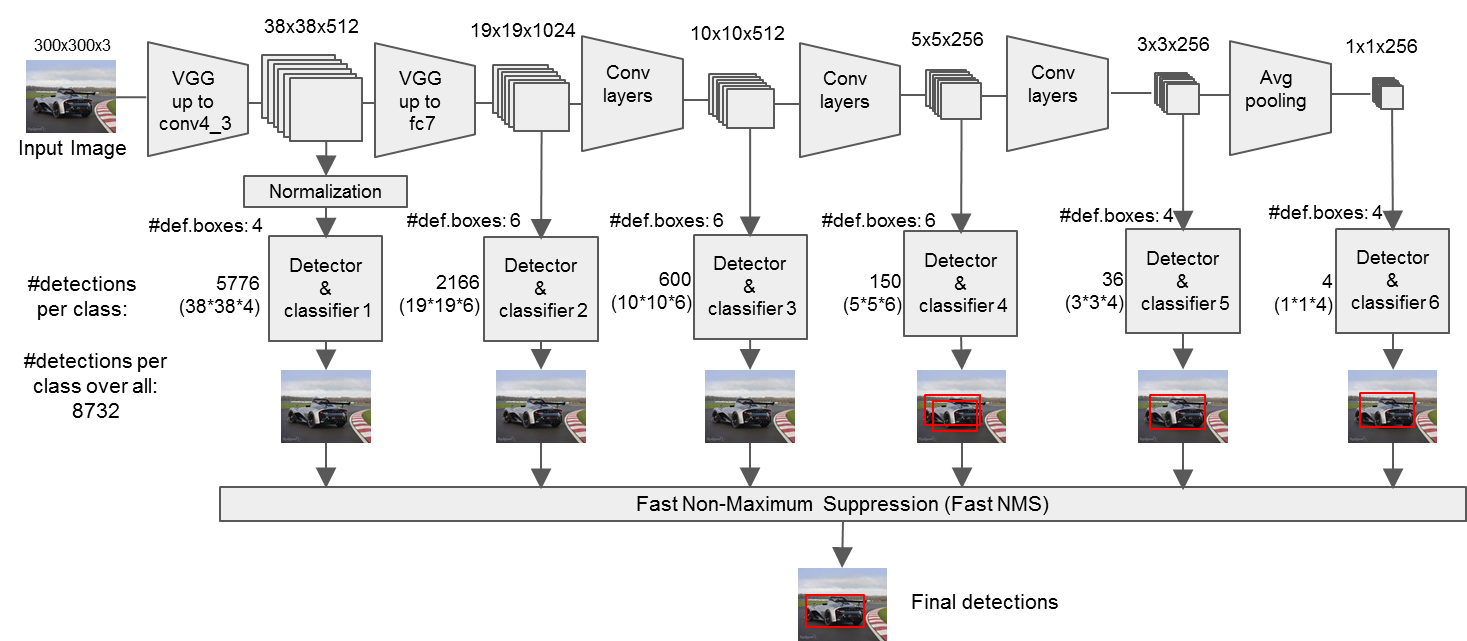
\includegraphics[width=1\textwidth]{figures/liucheng.png}
	\caption{多个特征层的协作}
\end{figure}
\subsection{先验框}
\par
SSD之所以提升了推理速度,很大一部分原因是其放弃了以前在原图上进行区域提议(region proposal)的操作,
SSD直接生成一系列先验框(default box),以先验框为初始的box,计算其与正确标注框(gound truth)的相对坐标,
之后对相对坐标进行编码,根据先验框位置再解码就可得到GT框。整个过程通过网络的一次前向传播即可完成。
在特征图上生成的先验框如下图\mycite{2016SSD}所示:
\begin{figure}[H]
	\centering
	\setlength{\abovecaptionskip}{0cm}  
	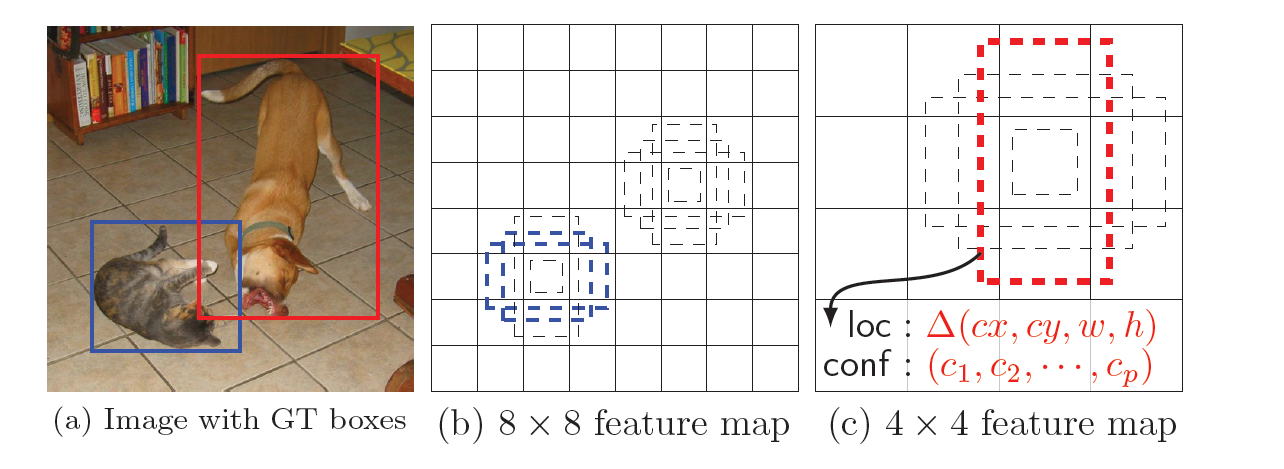
\includegraphics[scale=0.45]{figures/SSD.png}
	\caption{SSD的先验框}
\end{figure}
生成规则在\mycitex{2016SSD}中给出了具体的公式,此处不再提及。
\subsection{损失函数}
\par
SSD的损失函数包含两个部分,一个是定位损失$L_{loc}$,一个是分类损失$L_{conf}$,整个损失函数表达如下:
\[
L(x,c,l,g)=\frac{1}{N}(L_{conf}(x,c)+\alpha L_{loc}(x,l,g))
\]
\par
其中$N$是先验框正样本数量,$c$是类别置信度预测值,$l$是先验框对应的边界框预测值,$g$是ground truth的位置参数,
$x$代表网络的预测值。
\par
对于位置损失,采用Smooth L1 Loss,
位置信息都是encode之后的数值。而对于分类损失,
首先需要使用hard negtive mining将正负样本按照1:3 的比例把负样本抽样出来,
抽样的方法是:针对所有batch的confidence,按照置信度误差进行降序排列,
取出前top\_k个负样本。

\section{YOLO}
\par
接着介绍YOLO模型,其全称是You Only Look Once: Unified, Real-Time Object Detection,这也表明了Yolo算法的特点:只需要一次CNN运算,进行的是端到端的统一预测。YOLO有很多实现版本,这里以Yolo-v1\mycite{YOLO}为例,进行模型结构介绍。
\subsection{网络结构}
\par
Yolo网络结构,如下图\mycite{YOLO}所示:
\begin{figure}[H]
	\centering
	\setlength{\abovecaptionskip}{0cm}  
	\setlength{\belowcaptionskip}{0cm}  
	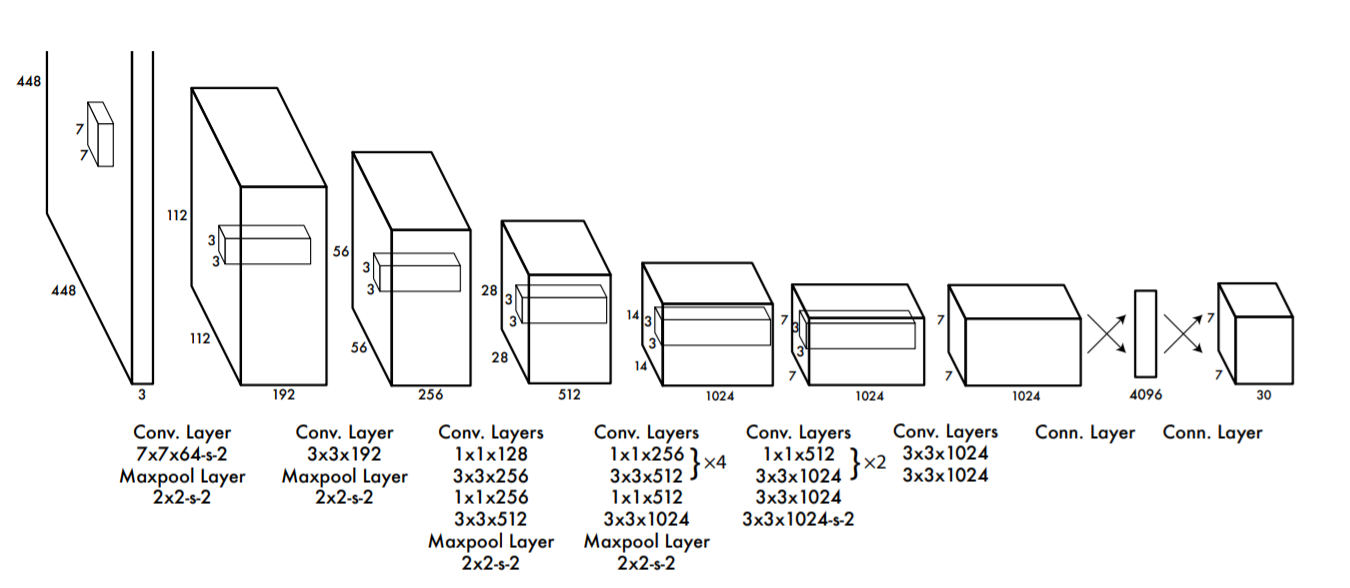
\includegraphics[width=1\textwidth]{figures/yolonet.png}
	\caption{Yolo网络结构}
\end{figure}
\par
可以看到,Yolo采用卷积网络来提取特征,然后使用全连接层来得到预测概率和坐标。网络结构中包含24个卷积层和2个全连接层。
其中卷积层,主要使用1x1卷积进行通道降维,然后紧跟3x3卷积提取特征。
对于卷积层和全连接层,不使用常见的ReLu激活函数,而是采用Leaky ReLU激活函数:$max(x,0.1x)$,但需要注意的是最终层仍使用线性激活函数ReLu。
\subsection{损失函数}
\par
类似地,检测在Yolo中也是回归问题,采用的是均方差损失函数。
整个算法的损失是由预测框的坐标误差,有无包含物体的置信度误差以及网格预测类别的误差三部分组成,三部分的损失都使用了均方误差的方式来实现。
具体表示如下:
\begin{equation}
	\begin{array}{l}
	\lambda_{\text {coord }} \sum_{i=0}^{S^{2}} \sum_{j=0}^{B} \mathbb{1}_{i j}^{\text {obj }}\left[\left(x_{i}-\hat{x}_{i}\right)^{2}+\left(y_{i}-\hat{y}_{i}\right)^{2}\right] \\
	\quad+\lambda_{\text {coord }} \sum_{i=0}^{S^{2}} \sum_{j=0}^{B} \mathbb{1}_{i j}^{\text {obj }}\left[\left(\sqrt{w_{i}}-\sqrt{\hat{w}_{i}}\right)^{2}+\left(\sqrt{h_{i}}-\sqrt{\hat{h}_{i}}\right)^{2}\right] \\
	+\sum_{i=0}^{S^{2}} \sum_{j=0}^{B} \mathbb{1}_{i j}^{\text {obj }}\left(C_{i}-\hat{C}_{i}\right)^{2} \\
	+\lambda_{\text {noobj }} \sum_{i=0}^{S^{2}} \sum_{j=0}^{B} \mathbb{1}_{i j}^{\text {noobj }}\left(C_{i}-\hat{C}_{i}\right)^{2} \\
	+\sum_{i=0}^{S^{2}} \mathbb{1}_{i}^{\text {obj }} \sum_{c \in \text { classes }}\left(p_{i}(c)-\hat{p}_{i}(c)\right)^{2}
	\end{array}
	\end{equation}
对于定位误差,采用较大的权重$\lambda_{coord}=5$。然后其区分不包含目标的边界框与含有目标的边界框的置信度.
对于前者,采用较小的权重值$\lambda_{noobj}=0.5$。其它权重值均设为1。对中心点直接进行均方误差,对宽高则使用平方根进行误差计算。
进行平方根均方误差的原因是较小的边界框中,定位误差要比较大的边界框要更敏感,为了区分这种不对等情况,所以对定位损失中的宽高损失加上了平方根。
\subsection{预测部分}
\par
以预测推理一张图片为例,Yolo输入图像后,输出7x7x30维度的张量,
即:将图片以物体中心点位置划分为7x7,每个单元格独立检测。
物体的中心落在哪个单元格,就由那个单元格负责预测。如下图\mycite{YOLO}所示:
\begin{figure}[H]
	\centering
	\setlength{\abovecaptionskip}{0cm}  
	\setlength{\belowcaptionskip}{0cm}  
	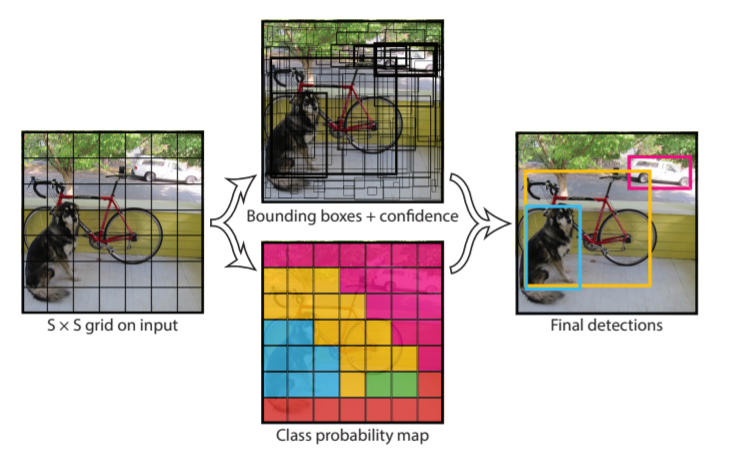
\includegraphics[width=1\textwidth]{figures/yologrid.png}
	\caption{Yolo检测方式}
\end{figure}
\par
最后张量维度为30,由(2*5+20)构成,其中2:每个单元格预测数量,5:$(x,y,w,h,score)$,20:模型可以预测20个种类。
\chapter{SNN模型结构}
\par
有两种方法可以改善通过转换获得的SNN的性能:一是在转换之前训练更好的ANN,二是通过消除SNN的近似误差来改善转换。后者在前一章节中给出了理论方法。而训练更好的ANN,目前用于目标检测且推理速度较快的模型主要是单阶段检测(one-stage detction):主要代表有ssd和yolo两类,因此我们选用这两类作为转换前的基础ANN
\section{spiking-ssd}
\par
首先介绍在ssd上进行的脉冲神经网络转化,即借用ssd的网络模型进行脉冲转化操作,
我们称之为"spiking-ssd"。ssd的具体结构我们已经在第三章中讲过,以下主要是阐述我们进行转化的网络模型。
\par
转换的核心是用脉冲神经元的脉冲发放频率代替人工神经网络中的激活值。
主要步骤如下:首先使用反向传播算法训练ANN(即ssd)达到较好性能,
然后将ANN中的BatchNorm层与前一层的卷积层进行融合,
根据每层的等效最大值对权重和偏置进行归一化,
并映射到具有相同拓扑结构的脉冲神经网络中,确保转换过程的信息损失最小。
实验方法流程如下图:
\begin{figure}[H]
	\centering
	\setlength{\abovecaptionskip}{0cm}  
	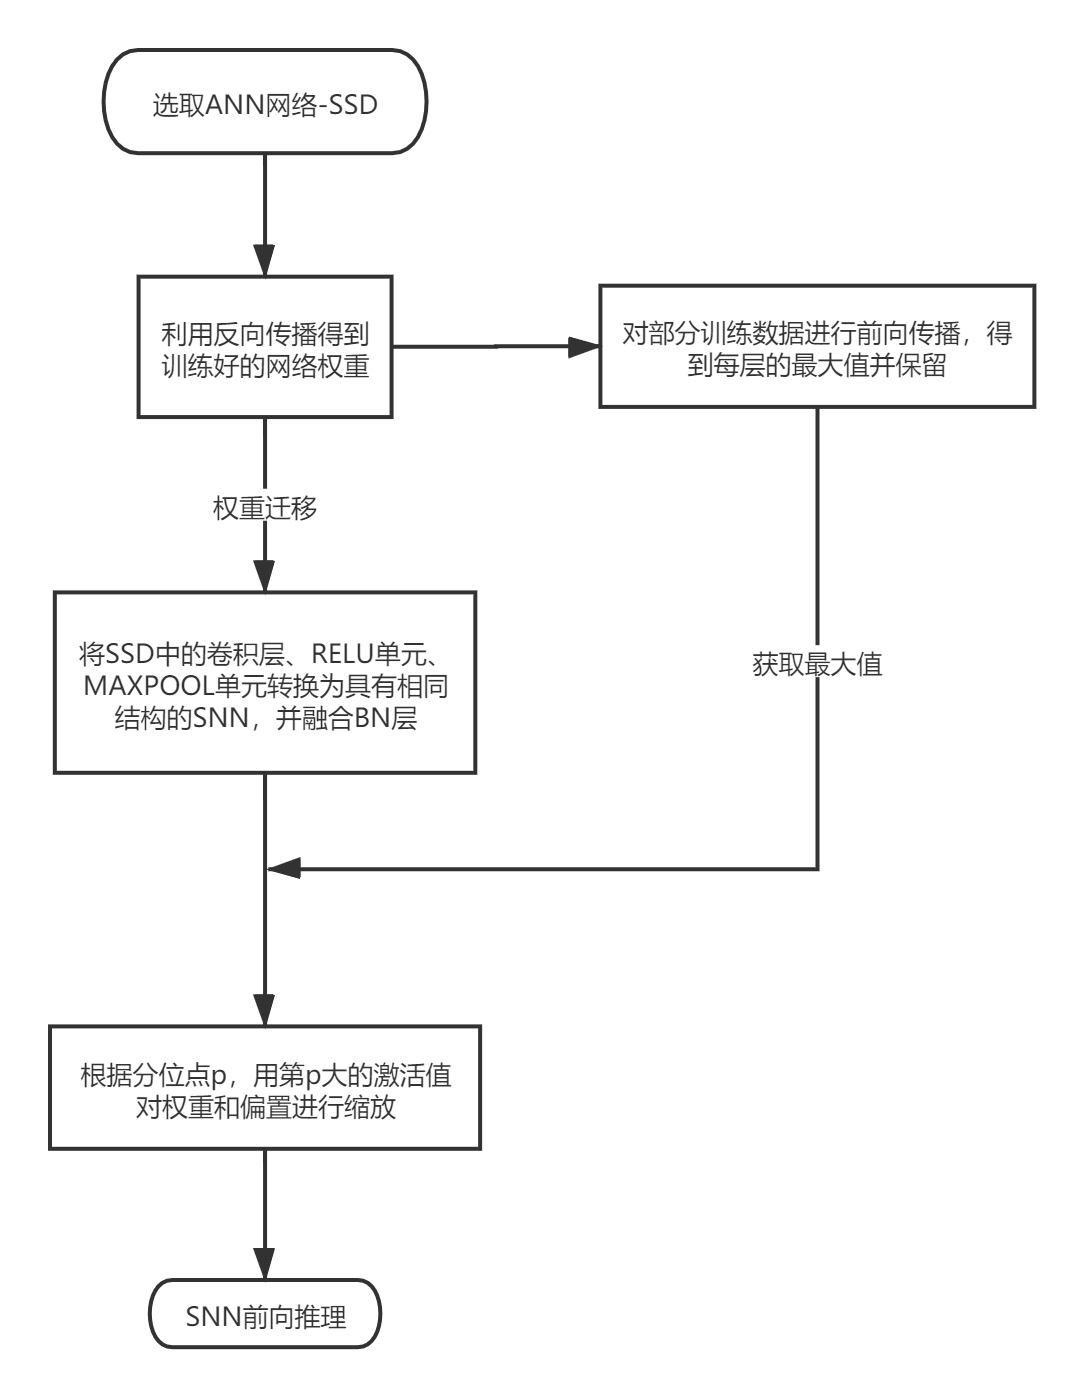
\includegraphics[scale = 0.35]{figures/flowchart.png}
	\caption{实验流程}
\end{figure}
\subsection{获取最大激活值}
\par
根据
\mycitex{2015Fast}提出的$\mathbf{Data-Base\; Normalization}$方法,
由于训练集和测试集服从同一分布,所以从训练集中选出部分图片,用这些图片作为输入,
输入到网络中进行前向传播,获得每一层的最大值,这就是max-norm的方法。实验时,
我们按前文所提到的设置一个百分位数p,
取p值在[99.0,99.999]范围内,选取第p大的激活值,防止个别过大的离群激活值导致发放率过低。
\subsection{等价转换操作}
\par
将原有SSD的四个模块Vgg、Extras、Loc、Conf均等价转换为脉冲单元SpikeUnit,
spikeUnit接收的opration类型有 nn.Conv2d/nn.Linear/nn.BatchNorm2d/nn.MaxPool2d/
nn.AvgPool2d/nn.Dropout/nn.ReLU,conv做运算并且发放脉冲,relu不做运算,而是单纯的积累膜电势并发放脉冲。
Maxpooling取最大的区域内的活动,只允许最大发放率的脉冲通过。
\subsection{前向推理}
\par
当网络转换完毕后,对输入的图片进行处理后,进入网络进行前向传播,即可得到目标置信度和位置的预测值。
这里的神经元采用IF神经元,实值编码,即将脉冲整数转换为浮点数,同时保留膜电势。
多个图片进行推理时,为了前面图片不影响后者图片,对各层中各个神经元进行膜电势、脉冲数、发放脉冲数的重置。
\section{spiking-yolo}
\par
在目标检测任务中,识别多个目标并在它们周围绘制边界框(回归问题)需要高数值精度来预测输出值。当使用常规ANN-SNN转换方法应用于SNN时,其遭受严重的性能降级。
可能的原因有两个:来自分层归一化导致的极低的发放率,以及leaky-RELU功能的中负激活没有办法表示。为此有两种新方法:分别为通道标准化和不平衡阈值的带符号神经元。
\subsection{通道标准化}
\par
为了防止神经元过度激活或过激活,基于数据的标准化技术被提出。逐层归一化\mycitex{2015Fast}(layer-norm)是最着名的技术之一:
基于训练和测试数据集的分布相似的假设,通过运行训练计算出的相应层的最大激活来规范特定层中的权重ANN中的数据集。公式前文中也提及:
\[
\mathbf{W}^l \to \mathbf{W}^l \frac{\lambda^l}{\lambda^{l-1}} and \mathbf{b}^l \to \mathbf{b}^l / \lambda^l
\]
\par
之后\mycitex{2017Conversion}引入了一种方法,该方法通过最大激活的99.9百分位来标准化激活,这为异常值提供了鲁棒性,从而确保了神经元的充分运行。
然而,根据我们的分析,传统的基于数据的归一化方法在应用于对象检测时由于激活不足而遭受显着的性能降级。
因此,我们提出了一种更细粒度的归一化技术,称为信道方向归一化(缩写为信道规范),以便在深度SNN中实现快速有效的信息传输。
我们的方法通过最大可能的激活(第99.9百分位数)以通道方式归一化权重,而不是传统的分层方法,算法如下:

\begin{algorithm}[H]
	\caption{通道标准化}%算法名字
	\SetKwBlock{Begin}{}{end}
	//从训练数据集中的每个通道中,计算最大激活值($\lambda$) \\
	\LinesNumbered %要求显示行号
\For{第 $l$ 层}{
    \For{第 $j$ 输出层}{
		 $\lambda_j^l=max(A_J^l)$ \\
	}
}
	//将通道标准化应用到测试集的推理上 \\
	\For{第 $l$ 层}{
    \For{第 $j$ 输出层}{
		 $\tilde{b}_j^l = b_j^l \; / \; \lambda _j ^l$
		\For{第 $i$ 输入通道}{
			\eIf{$l$ 是第一层}{
				$\tilde{w}_{i,j}^l=w_{i,j}^l \; / \; \lambda_j^l$
			}{
				$\tilde{w}_{i,j}^l=w_{i,j}^l \; / \; \lambda_j^l \; \lambda_i^{l-1}$
			}
		}
	}
}
\end{algorithm}
\par
细化的通道归一化可以提高神经元的发放率,即非常小的激活值被正确归一化,将在更短的时间内准确地传输信息。
实验证明逐通道归一化会使更多的神经元产生大量的脉冲。许多神经元产生高达80%的发放率。这是在逐层归一化上的发放率的很大改进。
这些小的激活可能意义不大,并且在诸如图像分类的简单应用中对网络的最终输出可能具有非常小的影响。但是,小的激活对回归问题至关重要。
\subsection{不平衡阈值的带符号神经元}
\par
ReLU是最常用的激活函数之一,仅保留正输入值,并丢弃所有负值; 
$x>0$时为$f(x)=x$,否则为$f(x) = 0$。与ReLU不同,leaky-ReLU包含具有泄漏项的负值,斜率为α,通常设置为0.01; 
$x>0$时为$f(x)=x$,否则为$f(x) = \alpha x$.
大多数先前的研究都集中在将IF(整合和反射)神经元转换为ReLU功能,并完全忽略了泄漏项。
也就是说,一旦可能包含有用信息的神经元变为负数,那么它将为零,并且所包含的信息在整个网络过程中将是无用的。
但在yolo中,泄露项占了不少的比例,因而不能忽视它,这里提出不平衡阈值的带符号神经元来表示漏项。
\par
可以引入第二个阈值电压$V_{th,neg}$,其等于正阈值电压除以一个负斜率$-\alpha$。公式如下:
\begin{equation}
	fire=(V_{mem}) = \begin{cases}
		1, & \text{if } V_{mem} \ge V_{th,pos}(V_{th}) \\
		-1, & \text{if } V_{mem} \le V_{th,neg}(-\frac{1}{\alpha}V_{th}) \\
		0, & \text{otherwise, no firing}
	\end{cases}
\end{equation}
\par
举个例子,如果$\alpha=0.1$,正激活阈值$V_{th,pos}$为1,则负激活阈值$V_{th,neg}$为-10。也就是负值时的膜电势需要十倍才能超过负阈值,产生脉冲。通过引入额外的阈值电压
来实现泄露项,我们实现了脉冲的离散性,在生物上更合理。
图片展示如下:
\begin{figure}[H]
	\centering
	\setlength{\abovecaptionskip}{0cm}  
	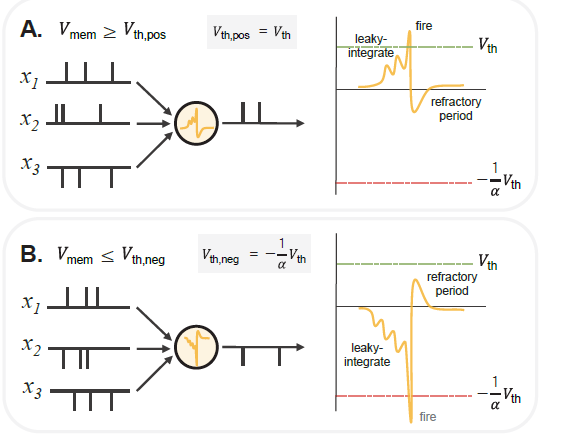
\includegraphics[scale=1]{figures/leakyrelu.png}
	\caption{带符号的不平衡阈值神经元}
\end{figure}
\subsection{解码方式}
\par
前面提到的两种方案,在后续的实验中,如果不应用带符号的不平衡阈值(IBT)神经元,很多的检测结果mAP都极低,
这是因为泄露RELU在tiny-yolo中占比很大。当仅应用具有IBT的带符号的神经元时,它仍然难以检测对象,
大约只有7.3%的mAP\mycite{Spiking-yolo},但这也表明带有IBT的带符号神经元可以补偿泄漏RELU中的泄漏项。
因此,接下来的实验将带有IBT方法的带符号神经元作为默认值来进行。这一部分主要是对解码方式进行讨论。
\par
有两种不同的输出解码方式:一种是基于累积膜电势$V_{mem}$,另一种基于脉冲计数$spike \;count$,脉冲计数$spike \;count$可以简单地由
$V_{mem}$除以$V_{th}$来计算。但是由于$V_{mem}$除以$V_{th}$的商是四舍五入的方式,因此可能出错并且丢失信息。所以基于$V_{mem}$的输出解码
方案在解释脉冲发放时会更加精确,在一些实验中证明\mycite{Spiking-yolo},其在通道和逐层归一化中也会更快地收敛。

\chapter{实验结果}
\section{数据集介绍}
\par
暂时空
\section{实验指标介绍}
\par
mAP(mean average precision)平均精度均值是目标检测中常用的指标,该指标可以
可以用来度量模型预测框类别和位置是否准确。在Pascal VOC中,
计算mAP的方式是取所有类别的AP的均值作为mAP的值。即:
\[
mAP=\frac{1}{N}\sum\limits_{i=1}^NAP_i
\]
而AP计算的方式是计算P-R(precision-recall)曲线下的面积(area under the curve, AUC)。
曲线的面积实际上可以转换为积分的求解。但在计算机中,我们是无法精确计算积分值的。
只能采取一些近似的方法。常用的积分求解方法就是插值法。以11点插值为例:
11点插值通过在recall轴采样11个等间隔的值[0,0.1,0.2,...,1.0],并对这11个recall值对应的precision值取平均来计算AP值。
\section{实验结果对比}
\subsection{ssd与spiking-ssd}
\par
在现有数据集下:选取数据集中56张图片作为测试集。以训练7000次保留的权重
$ssd300\_PIGFA\_5000.pth$进行预测,原始SSD表现如下:
{
\begin{center}
\begin{tabular}{rrrrrr}
	\hline
	dataset & recall & precision & F1 & AP@0.5 & mAP\\
	\hline
	pigfa & 1.0 & 1.0 & 1.0 & 1.0 & \multirow{4} *{0.95}\\
	pigma & 0.89 & 0.89 & 0.89 & 0.87 &\\
	peppa & 1.0 & 1.0 & 1.0 & 1.0 &\\
	george & 0.96 & 1.0 &0.98  & 0.96 &\\
	\hline
\end{tabular}
\end{center}
}
\par
同样,基于$ssd300\_PIGFA\_5000.pth$进行脉冲神经网络的转化,转换后的SSD表现如下:
{
\begin{center}
\begin{tabular}{rrrrrr}
	\hline
	dataset & recall & precision & F1 & AP@0.5 & mAP\\
	\hline
	pigfa & 0.26 & 0.43 & 0.32 & 0.18 & \multirow{4} *{0.65}\\
	pigma & 0.77 & 0.81 & 0.78 & 0.71 &\\
	peppa & 0.82 & 0.9 & 0.86 & 0.82 &\\
	george & 0.89 & 0.96 &0.89  & 0.89 &\\
	\hline
\end{tabular}
\end{center}
}

{
\begin{center}
\begin{tabular}{rrrrrr}
	\hline
	dataset & recall & precision & F1 & AP@0.5 & mAP\\
	\hline
	pigfa & 0.92 & 0.75 & 0.82 & 0.91 & \multirow{4} *{0.90}\\
	pigma & 0.91 & 0.91 & 0.91 & 0.89 &\\
	peppa & 1.0 & 1.0 & 1.0 & 1.0 &\\
	george & 0.89 & 0.92 &0.9  & 0.81 &\\
	\hline
\end{tabular}
\end{center}
}

{
\begin{center}
\begin{tabular}{rrrrrr}
	\hline
	dataset & recall & precision & F1 & AP@0.5 & mAP\\
	\hline
	pigfa & 0.92 & 0.92 & 0.92 & 0.91 & \multirow{4} *{0.91}\\
	pigma & 0.91 & 0.91 & 0.91 & 0.89 &\\
	peppa & 1.0 & 1.0 & 1.0 & 1.0 &\\
	george & 0.89 & 0.96 &0.92  & 0.83 &\\
	\hline
\end{tabular}
\end{center}
}
\par
目标检测中,效果取决于预测框的位置和类别是否准确,
mAP通过计算预测框和真实框的IoU来得到预测框的位置信息,
通过精确度和召回率指标来评价预测框的类别信息,
因此mAP是目前目标检测领域非常常用的评价指标。
\par
上面的结果显示,转换后的mAP降低了0.06,比原有的SSD降低了6\%,虽然理论上转换是接近无损的,但是不多的降低也是符合实际结果的。另外,此处的precision普遍较低,
因为精确率Precision反映的是预测出来准确结果占所有预测结果的准确性,结果中普遍较低,意味着检测结果有很多是错误类别,但因为有非极大值抑制的存在。
检测结果会进行删减,即不会影响mAP,这也是为什么回归率高的原因:代表预测出来准确结果在总体正样本中有很高的准确性。
\subsection{yolo与spiking-yolo}
\par
在现有的数据集下:选取数据集中划分的69张图片作为测试集。以最大训练次数8000次中最佳权重$best.pt$为权重进行预测,原始的Yolo表现如下:
{
\begin{center}
\begin{tabular}{rrrrrr}
	\hline
	dataset & recall & precision & F1 & AP@0.5 & mAP\\
	\hline
	pigfa & 1.0 & 0.974 & 0.987 & 0.995 & \multirow{4} *{0.99}\\
	pigma & 1.0 & 0.979 & 0.989 & 0.995 &\\
	peppa & 1.0 & 0.957 & 0.978 & 0.995 &\\
	george & 0.93 & 0.883 &0.905  & 0.974 &\\
	\hline
\end{tabular}
\end{center}
}

{
\begin{center}
\begin{tabular}{rrrrrr}
	\hline
	dataset & recall & precision & F1 & AP@0.5 & mAP\\
	\hline
	pigfa & 0.733 & 1.0 & 0.846 & 0.959 & \multirow{4} *{0.96}\\
	pigma & 0.728 & 1.0 & 0.842 & 0.9995 &\\
	peppa & 0.878 & 1.0 & 0.935 & 0.995 &\\
	george & 0.789 & 0.847 &0.817  & 0.9 &\\
	\hline
\end{tabular}
\end{center}
}

{
\begin{center}
\begin{tabular}{|r|r|r|r|r|r|}
	\hline
	\multicolumn{6}{|c|}{\textbf{Yolo}} \\
	\hline
	dataset & recall & precision & F1 & AP@0.5 & mAP\\
	\hline
	pigfa & 1.0 & 0.974 & 0.987 & 0.995 & \multirow{4} *{0.99}\\
	pigma & 1.0 & 0.979 & 0.989 & 0.995 &\\
	peppa & 1.0 & 0.957 & 0.978 & 0.995 &\\
	george & 0.929 & 0.883 & 0.905 & 0.974 &\\
	\hline
\end{tabular}
\end{center}
}
\par
同样,基于$best.pt$进行脉冲神经网络的转化,转换后的YOLO表现如下:
{
\begin{center}
\begin{tabular}{|r|r|r|r|r|r|}
	\hline
	\multicolumn{6}{|c|}{\textbf{Spiking-Yolo}} \\
	\hline
	dataset & recall & precision & F1 & AP@0.5 & mAP\\
	\hline
	pigfa & 0.733 & 1.0 & 0.846 & 0.959 & \multirow{4} *{0.96}\\
	pigma & 0.728 & 1.0 & 0.989 & 0.9995 &\\
	peppa & 0.878 & 1.0 & 0.935 & 0.995 &\\
	george & 0.789 & 0.847 & 0.817 & 0.9 &\\
	\hline
\end{tabular}
\end{center}
}
在我们的简单数据集上,转换的mAP接近原始yolo的值。
\chapter{总结讨论}
\section{数据对结果的影响}
\par
在Spiking-SSD中用到了$\mathbf{Data-Base\; Normalization}$的方法,这依赖于训练集中的部分数据,即使采用了0.9~0.99分位点避免一些特殊的离群值,但仍然要保证训练集和测试集服从同一分布,
否则得到的预测结果是不合理的。
\section{影响模型结果的几个因素}
\subsection{时间步长}
\par
在$2.2$节中提到,在仿真时间步长无限长的情况下,脉冲发放率才可以和模拟神经元的值进行近似,因此如果时间步长不足,则转换后模型的预测准确会受很大的影响。
但是如果追求无损的转换需要较高的时间步长,同样会增加了程序运行的时间。
经过实验,在Spiking-SSD和Spiking-Yolo中,时间步长设置为256可以较好地进行预测,这也是在时间和精度的一个折中。
\subsection{原始网络的效果}
\par
转换建立在ANN网络上,因此如果原始网络的训练没有收敛或者是损失没有降到一定的值,会出现ANN网络预测不好的问题,追求ANN近似的SNN自然也不会有好的预测结果,
因此高准确度的SNN网络,如果是通过转换实现的,需要原始的ANN有足够好的性能。
\subsection{转换单元的实现方式}
\par
同样是最大池化操作,现提出的方法有不同的脉冲实现方式。它们在模型上应用的结果也是不同的。
此外,如果不追求纯脉冲神经网络,只模拟部分激活值:另一部分如回归层、预测层仍由ANN实现,
这和纯脉冲操作实现的结果也是不同的。

\backmatter
\thesispagestyle{-4}{北京交通大学毕业设计(论文)}{}% 页眉设置

% 参考文献
%\bibliographystyle{ref/chinesebst}
%\bibliographystyle{plainnat,unsrt}
%\bibliographystyle{plainnat}
\bibliographystyle{elsarticle-num-names}
\bibliography{ref/refs}
\addcontentsline{toc}{chapter}{参考文献}

% 附录
\chapter*{附录一\qquad 英文原文}
\addcontentsline{toc}{chapter}{附录一\quad 英文原文}
% 英文原文
\chapter*{附录二\qquad 中文翻译}
\addcontentsline{toc}{chapter}{附录二\quad 中文翻译}
% 中文翻译


\end{document}
